%=================================================================
% Revised manuscript (MDPI template) based on revision_plan.md.
% Thesis version kept as main_ver0.tex.
% Build:  latexmk -pdf main_ver1.tex
%=================================================================
\documentclass[mathematics,article,submit,moreauthors]{Definitions/mdpi}

%=================================================================
% MDPI internal commands - do not modify
\firstpage{1}
\makeatletter
\setcounter{page}{\@firstpage}
\makeatother
\pubvolume{1}
\issuenum{1}
\articlenumber{0}
\pubyear{2026}
\copyrightyear{2026}
\datereceived{ }
\daterevised{ }
\dateaccepted{ }
\datepublished{ }

%=================================================================
% Packages and commands
\usepackage{bm}
\DeclareMathOperator*{\argmin}{arg\,min}
\DeclareMathOperator{\Var}{Var}
\DeclareMathOperator{\Cov}{Cov}
\DeclareMathOperator{\Corr}{Corr}
\DeclareMathOperator{\diag}{diag}
\newcommand{\E}{\mathbb{E}}
\newcommand{\Tw}{\mathcal{T}w}
\newcommand{\bmu}{\boldsymbol{\mu}}
\newcommand{\be}{\boldsymbol{e}}
\newcommand{\bc}{\boldsymbol{c}}
\newcommand{\bw}{\boldsymbol{w}}
\newcommand{\bx}{\boldsymbol{x}}
\newcommand{\bbeta}{\boldsymbol{\beta}}
\newcommand{\bpsi}{\boldsymbol{\psi}}
\newcommand{\boeta}{\boldsymbol{\eta}}
\newcommand{\bone}{\mathbf{1}}
\setlist[enumerate]{leftmargin=3em,labelsep=0.5em}

%=================================================================
\Title{Tweedie Evolutionary Credibility with Autoregressive Latent Risk: Closed-Form Premiums and Semi-Parametric GMM Estimation}

\newcommand{\orcidauthorA}{0000-0000-0000-000X}

\Author{Nahyun Kang and Himchan Jeong *}

\AuthorNames{Nahyun Kang and Himchan Jeong}

\address[1]{%
Department of Statistics and Actuarial Science, Simon Fraser University, Burnaby, BC V5A 1S6, Canada}

\corres{Correspondence: [e-mail to be added]}

%=================================================================
\abstract{%
Claim costs combine a mass at zero, a heavy right tail and serial dependence within policies. We develop evolutionary credibility for Tweedie claim costs in a GLM rating structure, where a multiplicative latent risk factor follows a second-order stationary process. For any latent autocovariance $\gamma(k)$, the best linear premium is the GLM premium times a closed-form credibility factor that depends only on $\gamma(\cdot)$ and a single nugget constant; the naive premium and the exact Tweedie credibility of Ohlsson and Johansson (2006) are special cases. For autoregressive latent risk, the premium has an updating-type Kalman recursion with positive weights; it is always positive, and the maximal bonus is bounded by the persistence parameter. Because every input is identified by second moments of standardized residuals, we propose a semi-parametric two-step GMM estimator that requires no distributional assumption on the latent process. The estimator comes with stage-1-corrected standard errors, a Hansen specification test and Wald tests of static versus evolutionary credibility. In simulations with estimated parameters, the feasible premium captures 80--97\% of the oracle gain whenever latent heterogeneity is non-negligible, and a fitted static premium is never materially worse than the naive premium. Interval estimates of the latent variance are less reliable when the latent signal is weak or the residuals are very heavy-tailed.}

\keyword{evolutionary credibility; Tweedie distribution; latent autoregressive process; Kalman filter; generalized method of moments; bonus--malus; experience rating}

\MSC{62P05; 91G05; 62M10; 62F12}

%=================================================================
\begin{document}

%=================================================================
\section{Introduction}\label{sec:intro}

Insurance claim costs have a large mass at zero, a heavy right tail and a variance that grows with the mean. The Tweedie compound Poisson--gamma family with power parameter $1<p<2$ captures all three features in a single exponential dispersion model and, combined with a log-link generalized linear model (GLM), is a standard tool for pricing with observable rating factors \citep{jorgensen1987,jorgensen1994fitting,smyth2002fitting,klugman2019}. Rating factors leave persistent unexplained heterogeneity, and experience rating, or credibility, uses each policyholder's claim history to correct the GLM premium \citep{buhlmann2005course}.

Classical credibility treats the latent risk of a policyholder as constant over time, so past years are exchangeable and receive equal weight. In practice, driving habits, occupation, health and exposure change, so the latent risk evolves. Recent experience is then more informative than old experience. Evolutionary credibility models make this explicit by letting the latent risk follow a stationary process \citep{gerber1975,sundt1981,albrecht1985,buhlmann2005course}. In frequency models with autoregressive random effects, the resulting premiums discount the age of claims \citep{pinquet2001,bolance2003}.

This paper develops evolutionary credibility for Tweedie claim costs inside a GLM rating structure. Conditional on a multiplicative latent factor $\theta_{it}$ with mean one, the claim cost $Z_{it}$ of policyholder $i$ in year $t$ is Tweedie with mean $\mu_{it}\theta_{it}$, where $\mu_{it}=\exp(\bx_{it}^\top\bbeta)$. The latent factor is only assumed to be second-order stationary with autocovariance $\gamma(k)$. The contributions are as follows.
\begin{enumerate}
\item \textbf{A closed-form premium for any stationary latent process (Theorem~\ref{thm:main}).} The best linear predictor of next year's claim cost is the GLM premium times a credibility factor computed from $\gamma(\cdot)$ and a single nugget constant $a=\phi\,\E[\theta^p]$. The within-policy noise enters through a heteroscedastic, covariate-dependent diagonal term $a\mu_{it}^{p-2}$. The independent, exchangeable (static), $\theta$-scale AR(1) and log-normal AR(1) cases are corollaries. The exchangeable case reproduces the Tweedie credibility estimator of \citet{ohlsson2006exact}.
\item \textbf{Structural results for AR(1) dependence (Proposition~\ref{prop:kalman}).} The premium has an updating-type (Kalman) recursion that costs $O(T)$ operations per policy. All weights are positive and add up to less than the autoregressive parameter $\rho$. The premium is therefore always positive, and the maximal bonus is bounded by $\rho$. We also give conditions under which recent years receive more weight than older ones, and show that this ordering can fail when the GLM mean changes over time.
\item \textbf{Semi-parametric GMM estimation and tests (Section~\ref{sec:estimation}).} Every input of the premium is identified by second moments of the standardized residuals $e_{it}=Z_{it}/\mu_{it}-1$. Our two-step generalized method of moments (GMM) estimator needs no distributional assumption on the latent process. It has closed-form, precision-weighted moments, stays inside the parameter space, and comes with a sandwich variance that corrects for first-stage estimation of $\bbeta$. It also provides a \citet{hansen1982} specification test and Wald tests of static versus evolutionary credibility and of no dependence.
\item \textbf{Simulation evidence with estimated parameters (Section~\ref{sec:simulation}).} A simulation study with time-varying covariates shows that the estimator is accurate, the tests have close to nominal size, and the feasible premium recovers most of the gain of the infeasible oracle-parameter premium. Exact population mean squared errors serve as a unit test of the simulation engine.
\end{enumerate}

The paper is organized as follows. Section~\ref{sec:literature} reviews related work. Section~\ref{sec:model} presents the model. Section~\ref{sec:premium} derives the premium and its properties. Section~\ref{sec:estimation} develops estimation and inference, and Section~\ref{sec:simulation} reports the simulation study. Section~\ref{sec:discussion} concludes. Proofs and computational details are in the appendices.

%=================================================================
\section{Related Literature}\label{sec:literature}

\textbf{Tweedie models and credibility.} Tweedie GLMs are widely used for pure premiums because the compound Poisson--gamma representation produces exact zeros and continuous positive amounts \citep{jorgensen1994fitting,smyth2002fitting}. \citet{jewell1974credible} showed that linear credibility is exact Bayesian for conjugate exponential families. \citet{ohlsson2006exact} extended exactness to Tweedie models with a multiplicative random effect. The resulting credibility weights are proportional to $\mu^{2-p}$, the natural Tweedie weights. Related work includes bonus--malus systems with separate frequency and severity components \citep{frangos2001design}, Tweedie models with distribution-free random effects \citep{ma2018tweedie}, multivariate Tweedie credibility \citep{jeong2024tweedie} and orderings of credibility factors \citep{ahn2021ordering}. These works treat the latent effect as constant over time.

\textbf{Evolutionary credibility.} \citet{gerber1975} introduced credibility formulas of the updating type, and \citet{sundt1981} developed recursive credibility estimation. In these, the premium is revised each year from the previous premium and the latest observation, which is a Kalman filter. \citet{albrecht1985} derived credibility for Poisson claim counts driven by a weakly stationary latent sequence, with recursive formulas for the coefficients. This is the closest antecedent of Theorem~\ref{thm:main}. Chapter~9 of \citet{buhlmann2005course} presents evolutionary models and their recursive (Kalman) computation in general. \citet{pinquet2001} modelled the age of claims in bonus--malus systems. \citet{bolance2003} estimated and tested autoregressive specifications of random effects in frequency models by moment methods, which is the spirit of our Section~\ref{sec:estimation}. \citet{pinquet2020} studied positivity of credibility weights under long-memory ARFIMA$(0,d,0)$ specifications, which is related to our Proposition~\ref{prop:kalman}. \citet{taylor2018} extended evolutionary credibility to hierarchical structures.

\textbf{Dependence in insurance losses.} Copula and multilevel models capture dependence across coverages and over time \citep{shi2016insurance,frees2016multivariate}. Multivariate Tweedie constructions have been used for capital and reserving \citep{furman2010multivariate,avanzi2016stochastic,alai2016multivariate}. These models describe dependence in the joint distribution of losses. Our focus is the design of linear credibility premiums that exploit the serial dependence of the latent risk.

\textbf{Positioning.} Relative to \citet{albrecht1985} and its successors, this paper adds four elements. First, the conditional response is Tweedie with power variance, so the nugget $a\mu_{it}^{p-2}$ is heteroscedastic and depends on covariates inside a GLM rating structure. Second, the exchangeable special case coincides exactly with \citet{ohlsson2006exact}. Third, we prove positivity and bonus bounds. Fourth, the GMM estimator needs no distributional assumption on $\theta$ and comes with tests of static versus evolutionary credibility. The paper builds on the first author's MSc project \citep{kang2026}.

%=================================================================
\section{Model}\label{sec:model}

\subsection{Notation and Assumptions}

Policyholders $i=1,\dots,I$ are observed in years $t=1,\dots,T_i$, and the target is year $T_i+1$. For exposition we take $T_i=T$; unbalanced panels are discussed in Section~\ref{sec:practical}. Table~\ref{tab:notation} collects the notation. Each symbol has one meaning throughout the paper. In particular, $(v,\rho)$ always refer to the $\theta$ scale, and $(\sigma_W^2,\rho_W)$ to the log scale.

\begin{table}[H]
\caption{Notation.\label{tab:notation}}
\begin{tabularx}{\textwidth}{l>{\raggedright\arraybackslash}X}
\toprule
\textbf{Symbol} & \textbf{Meaning} \\
\midrule
$\mu_{it}=\exp(\bx_{it}^\top\bbeta)$, $\bmu_i$ & GLM mean and its vector $(\mu_{i1},\dots,\mu_{iT})^\top$ \\
$\theta_{it}$ & latent multiplicative risk factor, $\E\theta_{it}=1$ \\
$v=\Var(\theta_{it})$ & latent variance ($\theta$ scale) \\
$\gamma(k)$, $r(k)=\gamma(k)/v$ & latent autocovariance $\Cov(\theta_{it},\theta_{i,t+k})$ and autocorrelation; $\gamma(0)=v$ \\
$a=\phi\,\E[\theta_{it}^p]$ & nugget (within-variance) constant \\
$q_{it}=\mu_{it}^{p-2}$ & nugget scale: $\Var(e_{it}\mid\boldsymbol\theta_i)$ has mean $a q_{it}$ \\
$e_{it}=Z_{it}/\mu_{it}-1$, $\be_i$ & standardized residual and its vector \\
$\Gamma_T=[\gamma(|t-s|)]_{t,s=1}^T$ & latent covariance matrix of years $1,\dots,T$ \\
$\bc_T=(\gamma(T),\dots,\gamma(1))^\top$ & latent cross-covariance with year $T+1$ \\
$D_{i}=\diag(a q_{i1},\dots,a q_{iT})$ & nugget matrix \\
$\rho$ & $\theta$-scale AR(1) parameter: $\gamma(k)=v\rho^k$ \\
$W_{it}=\log\theta_{it}$, $\sigma_W^2$, $\rho_W$ & log-scale variance and AR(1) parameter (log-normal AR(1) example) \\
\bottomrule
\end{tabularx}
\end{table}

\begin{Assumption}\label{ass:model}
For each policyholder $i$, conditional on the covariates:
\begin{enumerate}
\item[(A1)] $Z_{it}\mid\boldsymbol{\theta}_i\sim\Tw(\mu_{it}\theta_{it},\phi,p)$ with $1<p<2$, so that $\E[Z_{it}\mid\boldsymbol\theta_i]=\mu_{it}\theta_{it}$ and $\Var(Z_{it}\mid\boldsymbol\theta_i)=\phi(\mu_{it}\theta_{it})^p$. The $Z_{it}$ are conditionally independent over $t$ given the latent path $\boldsymbol\theta_i=(\theta_{i1},\theta_{i2},\dots)$.
\item[(A2)] $\theta_{it}>0$, $\E\theta_{it}=1$ and $\E\theta_{it}^2<\infty$.
\item[(A3)] $(\theta_{it})_t$ is second-order stationary: $\Cov(\theta_{it},\theta_{is})=\gamma(|t-s|)$ with $v=\gamma(0)>0$.
\item[(A4)] $\E[\theta_{it}^p]$ does not depend on $t$ (this holds, e.g., under strict stationarity).
\item[(A5)] Policyholders are mutually independent.
\end{enumerate}
\end{Assumption}

The normalization $\E\theta_{it}=1$ makes $\mu_{it}$ the marginal mean, $\E Z_{it}=\mu_{it}$, and separates the latent factor from the GLM intercept. By Jensen's and Lyapunov's inequalities, $1\le\E\theta^p\le(1+v)^{p-1}$ for $1<p<2$, so $a$ is finite under (A2). Assumptions (A1)--(A5) restrict only the first two moments of the latent process and the mean--variance relation of the response. No distributional assumption on $\theta$ is needed. As shown below, the fractional moment $\E\theta^p$ enters only through $a$, and $a$ is identified from the data.

\begin{Lemma}[Second-moment structure]\label{lem:moments}
Under Assumption~\ref{ass:model}, $\E e_{it}=0$ and
\begin{equation}\label{eq:moments}
\Cov(e_{it},e_{is})=\gamma(|t-s|)+\mathbb{1}\{t=s\}\,a\,q_{it},\qquad t,s\ge1 .
\end{equation}
\end{Lemma}

\begin{proof}
Write $e_{it}=x_{it}+\varepsilon_{it}$ with $x_{it}=\theta_{it}-1$ and $\varepsilon_{it}=(Z_{it}-\mu_{it}\theta_{it})/\mu_{it}$. By (A1), $\E[\varepsilon_{it}\mid\boldsymbol\theta_i]=0$, $\Var(\varepsilon_{it}\mid\boldsymbol\theta_i)=\phi\theta_{it}^p\mu_{it}^{p-2}$ and $\Cov(\varepsilon_{it},\varepsilon_{is}\mid\boldsymbol\theta_i)=0$ for $t\ne s$. Hence the $\varepsilon_{it}$ are uncorrelated with each other and with the latent path, and $\Var(\varepsilon_{it})=\phi\,\E[\theta_{it}^p]\,\mu_{it}^{p-2}=a q_{it}$ by (A4). The result follows from (A3).
\end{proof}

\subsection{Examples of Latent Processes}\label{sec:examples}

Any positive-semidefinite autocovariance $\gamma(\cdot)$ is allowed. The following cases are used below.
\begin{itemize}
\item \emph{Independence:} $\gamma(k)=0$ for $k\ge1$.
\item \emph{Exchangeable (static):} $\theta_{it}=\theta_i$, so $\gamma(k)=v$ for all $k$.
\item \emph{$\theta$-scale AR(1):} $\gamma(k)=v\rho^k$, $0\le\rho<1$. Any positive process with $\E[\theta_{t+1}\mid\theta_t,\theta_{t-1},\ldots]=1-\rho+\rho\theta_t$ has this autocovariance, for example the gamma autoregressive sequences of \citet{gaver1980}.
\item \emph{Log-normal AR(1):} $W_{it}=\log\theta_{it}$ is a stationary Gaussian AR(1) with variance $\sigma_W^2$, autocorrelation $\rho_W$ and mean $-\sigma_W^2/2$. Then
\begin{equation}\label{eq:logar1}
v=e^{\sigma_W^2}-1,\qquad \gamma(k)=\exp(\sigma_W^2\rho_W^k)-1,\qquad \E\theta^p=\exp\{\sigma_W^2p(p-1)/2\}.
\end{equation}
The $\theta$-scale autocorrelation $r(k)=\{\exp(\sigma_W^2\rho_W^k)-1\}/\{\exp(\sigma_W^2)-1\}$ is \emph{not} geometric. By convexity, $r(k)\le\rho_W^k$. For given $(v,r(1))$, the log-scale parameters are $\sigma_W^2=\log(1+v)$ and $\rho_W=\log\{1+v\,r(1)\}/\sigma_W^2$.
\item \emph{Other structures:} ARMA, long-memory (ARFIMA) and regime-switching processes for $\log\theta_{it}$ or for $\theta_{it}$. Each implies its own $\gamma(\cdot)$, and Theorem~\ref{thm:main} applies unchanged.
\end{itemize}

%=================================================================
\section{The Evolutionary Credibility Premium}\label{sec:premium}

\subsection{General Stationary Latent Processes}

We suppress the index $i$. Let $\mathcal{F}_T=\{Z_1,\dots,Z_T\}$, with the covariates $\bx_1,\dots,\bx_{T+1}$ treated as known. The (inhomogeneous) linear credibility premium is the best linear predictor
\[
P_{T+1}=\widehat{\alpha}_0+\sum_{t=1}^T\widehat{\alpha}_tZ_t,\qquad (\widehat\alpha_0,\dots,\widehat\alpha_T)=\argmin_{\alpha\in\mathbb{R}^{T+1}}\E\Big[\Big(Z_{T+1}-\alpha_0-\sum_{t=1}^T\alpha_tZ_t\Big)^2\Big].
\]

\begin{Theorem}\label{thm:main}
Under Assumption~\ref{ass:model}, the linear credibility premium for year $T+1$ is
\begin{equation}\label{eq:premium}
P_{T+1}=\mu_{T+1}\Big\{1+\bc_T^\top(\Gamma_T+D_T)^{-1}\be_T\Big\}=\mu_{T+1}\Big(1+\sum_{t=1}^Tw_te_t\Big),\qquad \bw=(\Gamma_T+D_T)^{-1}\bc_T,
\end{equation}
where $\Gamma_T=[\gamma(|t-s|)]_{t,s\le T}$, $D_T=\diag(a\mu_1^{p-2},\dots,a\mu_T^{p-2})$, $\bc_T=(\gamma(T),\dots,\gamma(1))^\top$ and $\be_T=(e_1,\dots,e_T)^\top$. The mean squared error is
\[
\E(Z_{T+1}-P_{T+1})^2=\mu_{T+1}^2\big\{v+a\mu_{T+1}^{p-2}-\bc_T^\top(\Gamma_T+D_T)^{-1}\bc_T\big\}.
\]
\end{Theorem}

\begin{proof}
Since $Z_t=\mu_t(1+e_t)$ with known $\mu_t$, linear predictors in $(1,Z_1,\dots,Z_T)$ and in $(1,e_1,\dots,e_T)$ coincide. Because $\E\be_T=\boldsymbol0$, the best linear predictor of $e_{T+1}$ given $\be_T$ is
\[
\Cov(e_{T+1},\be_T)\,\Var(\be_T)^{-1}\be_T .
\]
 By Lemma~\ref{lem:moments}, $\Var(\be_T)=\Gamma_T+D_T$, which is positive definite because $\Gamma_T$ is positive semi\-definite and $D_T$ has a positive diagonal. Also $\Cov(e_{T+1},e_t)=\gamma(T+1-t)$. Multiplying by $\mu_{T+1}$ gives \eqref{eq:premium}, and the MSE is the usual prediction error variance.
\end{proof}

The premium is a multiplicative experience correction to the GLM premium. The weight of each past year depends on the covariance of the latent risk with year $T+1$ and on the precision of that year's experience. A year with a large expected claim cost $\mu_t$ has a smaller nugget $a\mu_t^{p-2}$, because $p<2$, and therefore carries more information about $\theta_t$.

\begin{Corollary}[Special cases]\label{cor:special}
\begin{enumerate}
\item[(i)] \textup{Independence.} If $\gamma(k)=0$ for $k\ge1$, then $P_{T+1}=\mu_{T+1}$, the naive (GLM) premium.
\item[(ii)] \textup{Exchangeable.} If $\gamma(k)=v$ for all $k\ge0$, then, with $\kappa=a/v$,
\begin{equation}\label{eq:static}
P_{T+1}=\mu_{T+1}\,\frac{\kappa+\sum_{t=1}^TZ_t\,\mu_t^{1-p}}{\kappa+\sum_{t=1}^T\mu_t^{2-p}}.
\end{equation}
This is the Tweedie credibility estimator of \citet{ohlsson2006exact}: a B\"uhlmann--Straub-type estimator with natural weights $\mu_t^{2-p}$ and credibility constant $\kappa$.
\item[(iii)] \textup{$\theta$-scale AR(1).} If $\gamma(k)=v\rho^k$, then $\bw=(R_T+v^{-1}D_T)^{-1}(\rho^T,\dots,\rho)^\top$ with $[R_T]_{ts}=\rho^{|t-s|}$.
\item[(iv)] \textup{Log-normal AR(1).} If $\log\theta_t$ is a Gaussian AR(1), \eqref{eq:premium} holds with $\gamma(k)$ and $a$ given by \eqref{eq:logar1}.
\end{enumerate}
\end{Corollary}

\begin{proof}
(i) $\bc_T=\boldsymbol0$. (ii) $\Gamma_T=v\bone\bone^\top$ and $\bc_T=v\bone$. By the Sherman--Morrison formula, $\bw=v D_T^{-1}\bone/(1+v\bone^\top D_T^{-1}\bone)$, so $w_t=\mu_t^{2-p}/(\kappa+\sum_s\mu_s^{2-p})$. Using $\mu_t^{2-p}(1+e_t)=Z_t\mu_t^{1-p}$ gives \eqref{eq:static}. (iii) and (iv) are direct substitutions.
\end{proof}

\begin{Remark}[Which moments of $\theta$ matter]\label{rem:moments}
The premium depends on the latent law only through $\gamma(\cdot)$ and the fractional moment $\E\theta^p$. The latter enters only through the product $a=\phi\,\E\theta^p$, which is identified from the diagonal second moments of $e_{it}$ (Section~\ref{sec:estimation}). Neither $\phi$ nor $\E\theta^p$ needs to be known separately, and no distributional assumption on $\theta$ is required. Formulas such as $\E\theta^p=(1+v)^{p(p-1)/2}$ hold only for specific constructions (here, a log-normal marginal with variance $v$) and are not used for estimation.
\end{Remark}

\subsection{AR(1) Dependence: Recursion, Positivity and Bounds}

For the $\theta$-scale AR(1) structure $\gamma(k)=v\rho^k$, write $x_t=\theta_t-1$ and $d_t=a\mu_t^{p-2}$. Then $\eta_t=x_{t+1}-\rho x_t$ is uncorrelated with $x_s$ for $s\le t$ and with every $\varepsilon_s$, and $\Var(\eta_t)=v(1-\rho^2)$. Hence
\[
x_{t+1}=\rho x_t+\eta_t,\qquad e_t=x_t+\varepsilon_t,\qquad \Var(\varepsilon_t)=d_t,
\]
is a linear state-space model in the second-order sense. The Kalman recursions therefore compute linear projections exactly, without any Gaussian assumption \citep[Chapter~12]{brockwell1991}; see also \citet{harvey1989}.

\begin{Proposition}\label{prop:kalman}
Let $\gamma(k)=v\rho^k$ with $0<\rho<1$, and let $d_t=a\mu_t^{p-2}>0$.
\begin{enumerate}
\item[(a)] \textup{Updating-type recursion.} Set $\hat x_1=0$, $V_1=v$ and, for $t=1,\dots,T$,
\[
K_t=\frac{V_t}{V_t+d_t},\qquad \hat x_{t+1}=\rho\{(1-K_t)\hat x_t+K_te_t\},\qquad V_{t+1}=\rho^2(1-K_t)V_t+(1-\rho^2)v .
\]
Then $P_{T+1}=\mu_{T+1}(1+\hat x_{T+1})$ coincides with \eqref{eq:premium}, and $V_{T+1}$ is the prediction MSE of $\theta_{T+1}$.
\item[(b)] \textup{Weights.} $w_t=\rho^{T+1-t}K_t\prod_{s=t+1}^{T}(1-K_s)>0$ for $t=1,\dots,T$.
\item[(c)] \textup{Total credibility.} $S_T=\sum_{t=1}^Tw_t$ satisfies $S_{t}=\rho\{(1-K_t)S_{t-1}+K_t\}$ with $S_0=0$, and $0<S_T<\rho$.
\item[(d)] \textup{Positivity and bonus bound.} $P_{T+1}\ge\mu_{T+1}(1-S_T)>(1-\rho)\mu_{T+1}>0$. The maximal bonus, attained by a claim-free history, is $S_T<\rho$, so the premium discount never exceeds $100\rho\%$. The malus is unbounded.
\item[(e)] \textup{Comparative statics.} Every gain $K_t$, the most recent weight $w_T=\rho K_T$ and the total credibility $S_T$ are nondecreasing in $v$. Because the weights depend on $(v,a,\bmu)$ only through $d_t/v$, the same holds under a proportional increase of all $\mu_t$.
\item[(f)] \textup{Recency.} If $d_t-d_{t-1}\le v(1-\rho)/\rho$ for $t=2,\dots,T$, then $w_1<w_2<\dots<w_T$. This holds, in particular, when $\mu_t$ is constant or nondecreasing in $t$. Without such a condition the ordering can fail.
\item[(g)] \textup{Limits and steady state.} As $\rho\to0$, $P_{T+1}\to\mu_{T+1}$. As $\rho\to1$, $P_{T+1}$ converges to the exchangeable premium \eqref{eq:static}, and the recursion becomes the B\"uhlmann--Straub recursion $V_{t+1}=(1-K_t)V_t$. If $d_t\equiv d$, then $K_t\to K^\ast=u^\ast/(u^\ast+\delta)$ with $\delta=d/v$ and
\[
u^\ast=\tfrac12\Big[-(1-\rho^2)(\delta-1)+\sqrt{(1-\rho^2)^2(\delta-1)^2+4(1-\rho^2)\delta}\,\Big].
\]
For long histories the premium is exponential smoothing: the weight of year $T+1-j$ tends to $\rho K^\ast\{\rho(1-K^\ast)\}^{j-1}$, and $S_T\to\rho K^\ast/\{1-\rho(1-K^\ast)\}<\rho$.
\end{enumerate}
\end{Proposition}

The proof is in Appendix~\ref{app:proofs}. Part (d) has two practical consequences. The fitted premium is always strictly positive, so the Tweedie deviance is always defined. The persistence parameter $\rho$ also directly caps the bonus a claim-free history can earn. Part (f) is the ``age of claims'' property of \citet{pinquet2001}. A counterexample to unrestricted recency is $T=2$, $v=0.5$, $\rho=0.8$, $d=(0.01,25)$: an old year with a large expected cost (small nugget) receives weight $w_1=0.623$, while a recent year with a small expected cost receives $w_2=0.006$. Part (e) is in the spirit of the orderings of credibility factors in \citet{ahn2021ordering}. Individual older weights need not be monotone in $v$, because a larger $v$ also shifts weight toward recent years.

For a general $\gamma(\cdot)$, the Durbin--Levinson or innovations algorithm provides an analogous $O(T^2)$ recursion \citep[Chapter~5]{brockwell1991}. Positivity of the weights is then not guaranteed for non-monotone autocovariances \citep[cf.][]{pinquet2020}. Under the log-normal AR(1) structure, positivity held in all our simulated portfolios, but this is an empirical observation rather than a theorem.

%=================================================================
\section{Semi-Parametric Estimation and Inference}\label{sec:estimation}

\subsection{Moment Identities and Identification}

By Lemma~\ref{lem:moments}, the standardized residuals satisfy
\begin{align}
\E[e_{it}e_{i,t+k}\mid\bx_i]&=\gamma(k), && k=1,\dots,T-1, \label{eq:lagmom}\\
\E[e_{it}^2\mid\bx_i]&=\gamma(0)+a\,q_{it}, && q_{it}=\mu_{it}^{p-2}. \label{eq:diagmom}
\end{align}
The lag moments \eqref{eq:lagmom} do not depend on $\phi$, $p$ or the law of $\theta$. The premium \eqref{eq:premium} depends on the data-generating process only through $(\bbeta,p)$, $\gamma(0),\dots,\gamma(T)$ and $a$. Hence:
\begin{itemize}
\item $\gamma(1),\dots,\gamma(T-1)$ are identified nonparametrically by \eqref{eq:lagmom};
\item $\gamma(0)$ and $a$ are identified separately by \eqref{eq:diagmom} whenever $\mu_{it}^{p-2}$ varies across observations, which is the case with any nontrivial rating structure;
\item $\gamma(T)$, which enters $\bc_T$, cannot be identified nonparametrically from a $T$-year panel and requires a parametric structure or an extrapolation rule.
\end{itemize}

\subsection{Two-Step Estimator}

\textbf{Stage 1: mean structure.} Fit the Tweedie quasi-likelihood GLM under working independence, i.e., solve $\sum_{i,t}\bx_{it}(Z_{it}-\mu_{it})\mu_{it}^{1-p}=\boldsymbol0$. The estimator $\widehat\bbeta$ is consistent because $\E Z_{it}=\mu_{it}$ \citep{wedderburn1974}, whatever the serial dependence. Set $\hat\mu_{it}=\exp(\bx_{it}^\top\widehat\bbeta)$, $\hat e_{it}=Z_{it}/\hat\mu_{it}-1$ and $\hat q_{it}=\hat\mu_{it}^{p-2}$.

\textbf{Stage 2: weighted moment contributions.} Collect the second-moment parameters in
\[
\boeta=(\gamma(0),a,\gamma(1),\dots,\gamma(T-1))^\top\in\mathbb{R}^{T+1}.
\]
The per-policy moment contributions are
\begin{align}
g_{ik}(\boeta)&=\sum_{t=1}^{T-k}w_{itk}\{\hat e_{it}\hat e_{i,t+k}-\gamma(k)\}, && k=1,\dots,T-1,\label{eq:g}\\
h_{ij}(\boeta)&=\sum_{t=1}^{T}\omega_{it}\,z_{itj}\{\hat e_{it}^2-\gamma(0)-a\hat q_{it}\}, && \boldsymbol z_{it}=(1,\hat q_{it})^\top,\label{eq:h}
\end{align}
with precision weights
\[
w_{itk}=(\hat s_{it}^2\,\hat s_{i,t+k}^2)^{-1},\qquad \omega_{it}=\hat s_{it}^{-4},\qquad \hat s_{it}^2=\hat a\,\hat q_{it}+\hat v .
\]
Here $\hat s_{it}^2$ estimates $\Var(e_{it})$. The weights are computed from preliminary estimates and updated two or three times, starting from equal weights. They down-weight policy-years with small $\mu_{it}$, whose residuals consist mostly of Tweedie noise. This matters when $\mu$ is very heterogeneous. Since the weights depend only on covariates and preliminary estimates, they do not affect consistency.

Let $\boldsymbol m_i(\boeta)=(h_{i1},h_{i2},g_{i1},\dots,g_{i,T-1})^\top$ and $\bar{\boldsymbol m}(\boeta)=I^{-1}\sum_i\boldsymbol m_i(\boeta)$. The moments are \emph{linear} in $\boeta$, so $\bar{\boldsymbol m}(\boeta)=\bar{\boldsymbol b}-\bar A\boeta$ for a block-diagonal matrix $\bar A$ and a vector $\bar{\boldsymbol b}$ of weighted sums. The \emph{nonparametric} (NP) estimator solves $\bar{\boldsymbol m}(\widehat\boeta)=\boldsymbol0$ in closed form: each $\hat\gamma(k)$ is a weighted average of lag-$k$ cross-products, and $(\hat\gamma(0),\hat a)$ is a weighted regression of $\hat e_{it}^2$ on $(1,\hat q_{it})$.

\textbf{Parametric latent structures.} A structure $\boeta=\boeta(\bpsi)$ specifies $\gamma(k;\bpsi)$ and $a$. We use
\begin{itemize}
\item S0 (independence, naive): $\gamma(k)=0$ for $k\ge1$;
\item S1 ($\theta$-scale AR(1)): $\bpsi=(v,\rho,a)$, $\gamma(k)=v\rho^k$; Proposition~\ref{prop:kalman} applies;
\item S2 (log-normal AR(1)): $\bpsi=(\sigma_W^2,\rho_W,a)$, $\gamma(k)=\exp(\sigma_W^2\rho_W^k)-1$;
\item S3 (exchangeable): $\bpsi=(v,a)$, $\gamma(k)=v$, which gives a \emph{fitted} static benchmark through Corollary~\ref{cor:special}(ii);
\item NP: $\widehat\boeta$ itself, with the tail $\hat\gamma(T)=\hat\gamma(T-1)\min\{\hat\gamma(T-1)/\hat\gamma(T-2),1\}$ when both are positive, and $0$ otherwise.
\end{itemize}
The efficient two-step GMM estimator is
\begin{equation}\label{eq:gmm}
\widehat\bpsi=\argmin_{\bpsi}\ \bar{\boldsymbol m}(\boeta(\bpsi))^\top\,\widehat\Omega^{-1}\,\bar{\boldsymbol m}(\boeta(\bpsi)),
\end{equation}
where $\widehat\Omega$ is the covariance matrix of the per-policy contributions (clustered by policyholder) after the stage-1 correction below. Because $\bar{\boldsymbol m}$ is linear in $\boeta$, \eqref{eq:gmm} is equivalent to the minimum-distance problem
\begin{equation}\label{eq:md}
\widehat\bpsi=\argmin_{\bpsi}\ \{\widehat\boeta-\boeta(\bpsi)\}^\top\widehat V^{-1}\{\widehat\boeta-\boeta(\bpsi)\},\qquad \widehat V=I^{-1}\bar A^{-1}\widehat\Omega\bar A^{-\top}.
\end{equation}
All structures are therefore fitted to the same $T+1$ summary statistics with their estimated covariance, which is fast and numerically stable. We reparametrize $v=e^{\nu}$, $\sigma_W^2=e^{\nu}$, $\rho=\operatorname{logit}^{-1}(\kappa)$, $\rho_W=\operatorname{logit}^{-1}(\kappa)$ and $a=e^{\alpha}$, so that estimates always lie in the parameter space. We also report a \emph{lag-only} variant of S1, which fits $(v,\rho)$ to the lag moments \eqref{eq:lagmom} and takes $\hat a$ from the NP diagonal block, and an \emph{equal-weight} variant with $w_{itk}=\omega_{it}=1$.

\textbf{Plug-in premium.} The feasible premium inserts $\hat\mu_{i,T+1}$, $\hat e_{it}$, $\hat q_{it}$, $\gamma(k;\widehat\bpsi)$ and $\hat a$ into \eqref{eq:premium}, or into the recursion of Proposition~\ref{prop:kalman} for S1.

\subsection{Asymptotic Theory}

Let $\boldsymbol s_i(\bbeta)=\sum_t\bx_{it}(Z_{it}-\mu_{it})\mu_{it}^{1-p}$ be the stage-1 quasi-score and $S=\E\,\partial\boldsymbol s_i/\partial\bbeta^\top$. Stage 1 matters for inference: since $\partial e_{it}/\partial\bbeta=-\bx_{it}(1+e_{it})$, we have $\E\,\partial(e_{it}e_{is})/\partial\bbeta=-(\bx_{it}+\bx_{is})\gamma(|t-s|)\ne\boldsymbol0$ for $t\ne s$. Let $G_\beta=\E\,\partial\boldsymbol m_i/\partial\bbeta^\top$ and define the corrected contributions $\tilde{\boldsymbol m}_i=\boldsymbol m_i-G_\beta S^{-1}\boldsymbol s_i$. This is the influence function of the stacked estimator \citep[Section~6]{newey1994}.

\begin{Proposition}\label{prop:asy}
Suppose Assumption~\ref{ass:model} holds with $(\bx_i,\boldsymbol\theta_i,\boldsymbol Z_i)$ i.i.d.\ across $i$, $\E\theta_{it}^4<\infty$, bounded covariates and a nonsingular $\E[\sum_t\omega_{it}\boldsymbol z_{it}\boldsymbol z_{it}^\top]$. Let $T$ be fixed and $I\to\infty$. Then
\begin{enumerate}
\item[(i)] $\sqrt I(\widehat\boeta-\boeta_0)\to N(\boldsymbol0,V_\infty)$ with $V_\infty=\bar A^{-1}\Omega\bar A^{-\top}$ and $\Omega=\Var(\tilde{\boldsymbol m}_i)$;
\item[(ii)] if $\boeta_0=\boeta(\bpsi_0)$ with $\bpsi_0$ interior, $\boeta(\cdot)$ is injective and continuously differentiable, and $H=\partial\boeta/\partial\bpsi^\top$ has full column rank at $\bpsi_0$, then $\sqrt I(\widehat\bpsi-\bpsi_0)\to N(\boldsymbol0,(H^\top V_\infty^{-1}H)^{-1})$;
\item[(iii)] the Hansen statistic $J=\{\widehat\boeta-\boeta(\widehat\bpsi)\}^\top\widehat V^{-1}\{\widehat\boeta-\boeta(\widehat\bpsi)\}$ converges in distribution to $\chi^2_{T+1-\dim\bpsi}$.
\end{enumerate}
\end{Proposition}

\begin{proof}[Sketch]
(i) follows from a first-order expansion of $\bar{\boldsymbol m}(\widehat\boeta;\widehat\bbeta)=\boldsymbol0$ around $(\boeta_0,\bbeta_0)$ combined with $\widehat\bbeta-\bbeta_0=-S^{-1}I^{-1}\sum_i\boldsymbol s_i+o_p(I^{-1/2})$. The moment conditions hold for any weights that are functions of covariates, so estimating the weights does not affect the limit. (ii) and (iii) are standard results for optimal minimum distance and GMM \citep{hansen1982,newey1994}.
\end{proof}

In practice, $G_\beta$ is computed by numerical differentiation of $\bar{\boldsymbol m}$ with the weights held fixed, and $\widehat\Omega$ is the sample covariance of the $\tilde{\boldsymbol m}_i$. A policyholder-level (cluster) bootstrap is a simple alternative. Delta-method intervals for $v$ are formed on the log scale.

\subsection{Tests}\label{sec:tests}

\begin{itemize}
\item \emph{Specification.} The $J$ statistic of Proposition~\ref{prop:asy}(iii) tests a parametric structure, with $T-2$ degrees of freedom for S1 and S2 and $T-1$ for S3.
\item \emph{Static versus evolutionary credibility.} The Wald statistic for $H_0:\gamma(1)=\dots=\gamma(T-1)$, computed from the NP estimates, is asymptotically $\chi^2_{T-2}$. It does not require testing $\rho=1$ on the boundary of S1, and it does not involve the diagonal moments, so it is robust to misspecification of the variance function. In spirit it parallels the tests of \citet{bolance2003} for frequency models.
\item \emph{No dependence.} The Wald statistic for $H_0:\gamma(1)=\dots=\gamma(T-1)=0$ from the NP estimates is asymptotically $\chi^2_{T-1}$. The NP estimates are unrestricted, so there is no boundary problem. Testing $v=0$ within S1 requires the boundary theory of \citet{andrews1999}.
\end{itemize}

\subsection{Practical Extensions}\label{sec:practical}

\textbf{Choice of $p$.} The marginal variance is $\Var Z_{it}=a\mu_{it}^p+v\mu_{it}^2$, so a marginal Tweedie profile likelihood estimates a working value of $p$ that is biased toward 2. Instead, $p$ can be chosen to minimize the $J$ statistic of the diagonal moments \eqref{eq:diagmom} with the extra instrument $\hat q_{it}\log\hat\mu_{it}$ (one overidentifying restriction), or estimated jointly with $\boeta$. Sensitivity to $p$ should be reported; see Section~\ref{sec:sensitivity}.

\textbf{Exposure.} For pure premiums $Y_{it}=Z_{it}/\varpi_{it}$ with exposure $\varpi_{it}$ and $Y_{it}\mid\theta_{it}\sim\Tw(\mu_{it}\theta_{it},\phi/\varpi_{it},p)$, set $e_{it}=Y_{it}/\mu_{it}-1$. The diagonal moment becomes $\gamma(0)+a\mu_{it}^{p-2}/\varpi_{it}$, and $q_{it}$ and the weights change accordingly.

\textbf{Unbalanced panels.} Entry, exit and gaps need no special treatment. The sums in \eqref{eq:g}--\eqref{eq:h} run over observed years and observed pairs, and in \eqref{eq:premium} unobserved years are dropped. Equivalently, their nugget is set to infinity, which in Proposition~\ref{prop:kalman} means $K_t=0$.

\textbf{Computation.} The estimator requires one GLM fit, $O(IT^2)$ sums for the moment contributions and a low-dimensional minimum-distance problem. No numerical integration or MCMC is needed. For a portfolio of $I=10{,}000$ policies and $T=5$, the whole pipeline (GLM, moments, S1 fit and premiums) takes well under one second on a single CPU core.

%=================================================================
\section{Simulation Study}\label{sec:simulation}

\subsection{Design}\label{sec:design}

\textbf{Data-generating process.} Each replication simulates $I=2000$ policyholders over $T=5$ training years and one hold-out year $T+1$. Covariates are $\bx_{it}=(1,x_{1,it},x_{2,i})^\top$, where $x_{1,it}=b_i+u_{it}$ has a time-invariant part $b_i\sim N(0,0.6^2)$ and a time-varying part $u_{it}\sim N(0,0.8^2)$, and $x_{2,i}\sim\mathrm{Bernoulli}(0.5)$ is fixed over time. The GLM mean is $\mu_{it}=\exp(2.5+0.5x_{1,it}-0.5x_{2,i})$. Time-varying covariates exercise the time-varying nugget $a\mu_{it}^{p-2}$ that the premium is built for, and they help separate $v$ from $a$ in \eqref{eq:diagmom}. The latent factor follows the log-normal AR(1) model of Section~\ref{sec:examples}, and $Z_{it}\mid\theta_{it}\sim\Tw(\mu_{it}\theta_{it},\phi=10,p=1.5)$. The share of zero claims is $54$--$60\%$ across cells (Table~\ref{tab:exact}).

\textbf{Grid.} The grid is indexed by interpretable $\theta$-scale quantities: $v\in\{0.1,0.25,0.5,1\}$, with $v=2$ as a stress case, and $r(1)\in\{0.3,0.5,0.7,0.9\}$. Each pair maps to the log-normal AR(1) by $\sigma_W^2=\log(1+v)$ and $\rho_W=\log\{1+v\,r(1)\}/\sigma_W^2$. Under this data-generating process, S2 is correctly specified, whereas S1 is a (mildly) misspecified working model, because the $\theta$-scale autocorrelation is not exactly geometric. Each of the 20 cells uses 500 replications.

\textbf{Competitors.} All feasible methods use parameters estimated from the training years only.
\begin{itemize}
\item \emph{Naive}: the GLM premium $\hat\mu_{i,T+1}$.
\item \emph{Static (fitted)}: structure S3 and Corollary~\ref{cor:special}(ii). This is a fitted exchangeable model that estimates the covariance best matching the observed moments, not the full $\Var\theta$.
\item \emph{S1}: structure S1 and the recursion of Proposition~\ref{prop:kalman} (the main proposal).
\item \emph{S2} and \emph{NP}: structure S2 and the nonparametric autocovariances, plugged into Theorem~\ref{thm:main}.
\item \emph{S1 lag-only} and \emph{S1 equal weights}: the robustness variants of Section~\ref{sec:estimation}.
\item \emph{Oracle parameters}: Theorem~\ref{thm:main} with the true $(\bbeta,\gamma,a)$, i.e., the best linear premium.
\item \emph{Best exchangeable}: the best static premium with true moments (Appendix~\ref{app:mse}).
\item \emph{Oracle $\theta$}: $\mu_{i,T+1}\theta_{i,T+1}$, which is not a linear premium.
\end{itemize}

\textbf{Metrics.} For prediction, we report the paired relative reduction of out-of-sample MSE versus the naive premium, averaged over replications with Monte Carlo standard errors. We also report the share of the oracle gain,
\[
\text{share}(M)=\frac{\mathrm{PE}_{\rm naive}-\mathrm{PE}_M}{\mathrm{PE}_{\rm naive}-\mathrm{PE}_{\rm oracle\ param}},\qquad \mathrm{PE}_M=\E(\mu_{T+1}\theta_{T+1}-P^M_{T+1})^2,
\]
which uses the premium error to remove the irreducible Tweedie noise (Appendix~\ref{app:mse}); its standard error is computed by bootstrapping replications. We also report the fraction of replications in which a method beats the naive premium, and the mean Tweedie deviance. For estimation, we report medians and interquartile ranges (the sampling distributions are skewed), coverage of 95\% Wald intervals, rejection rates of the $J$ and Wald tests at the 5\% level, and the frequency of estimates near the boundary ($\hat\rho>0.99$ or $\hat v<10^{-3}$).

\textbf{Unit test.} Under correct moments the oracle-parameter premium is the best linear predictor. Its exact population MSE \eqref{eq:exactmse} is therefore a lower bound for every linear premium in expectation, and it must match the simulated oracle-parameter MSE within Monte Carlo error. Table~\ref{tab:exact} confirms this for all cells. In expectation, the ordering is oracle parameters $\le$ best exchangeable $\le$ naive.

\begin{table}[H]
\caption{Exact population quantities and the unit test. Zero: share of zero claims (\%). Exact MSE of the naive premium, and exact relative MSE reduction (\%) of the oracle-parameter premium (OP) and of the best exchangeable premium (BE) relative to naive. The last two columns compare the exact OP MSE with its simulated value (Monte Carlo SE in parentheses; 500 replications of $I=2000$).\label{tab:exact}}
\begin{adjustwidth}{-\extralength}{0cm}
\small
\begin{tabular*}{\fulllength}{@{\extracolsep{\fill}}cccccccc@{}}
\toprule
$v$ & $r(1)$ & Zero (\%) & Naive MSE & OP gain (\%) & BE gain (\%) & OP MSE (exact) & OP MSE (simulated) \\
\midrule
%BEGIN tab_exact
0.1 & 0.3 & 54 & 446.6 & 0.01 & 0.00 & 446.6 & 446.8 (2.1) \\
0.1 & 0.5 & 54 & 446.6 & 0.04 & 0.02 & 446.4 & 446.4 (2.1) \\
0.1 & 0.7 & 54 & 446.6 & 0.12 & 0.09 & 446.1 & 447.7 (2.2) \\
0.1 & 0.9 & 54 & 446.6 & 0.32 & 0.32 & 445.2 & 444.5 (2.0) \\
0.25 & 0.3 & 55 & 492.9 & 0.07 & 0.02 & 492.5 & 495.6 (2.8) \\
0.25 & 0.5 & 55 & 492.9 & 0.21 & 0.12 & 491.8 & 493.3 (2.8) \\
0.25 & 0.7 & 55 & 492.9 & 0.56 & 0.44 & 490.1 & 486.4 (2.6) \\
0.25 & 0.9 & 55 & 492.9 & 1.48 & 1.44 & 485.6 & 483.3 (2.7) \\
0.5 & 0.3 & 56 & 566.6 & 0.20 & 0.07 & 565.5 & 566.1 (3.9) \\
0.5 & 0.5 & 56 & 566.6 & 0.64 & 0.35 & 563.0 & 565.1 (3.8) \\
0.5 & 0.7 & 56 & 566.6 & 1.59 & 1.25 & 557.6 & 552.5 (3.5) \\
0.5 & 0.9 & 56 & 566.6 & 3.93 & 3.80 & 544.3 & 540.8 (3.5) \\
1 & 0.3 & 58 & 705.3 & 0.51 & 0.19 & 701.7 & 701.5 (7.3) \\
1 & 0.5 & 58 & 705.3 & 1.60 & 0.89 & 694.0 & 690.4 (5.9) \\
1 & 0.7 & 58 & 705.3 & 3.81 & 2.93 & 678.5 & 682.3 (6.3) \\
1 & 0.9 & 58 & 705.3 & 8.68 & 8.33 & 644.1 & 652.9 (6.3) \\
2 & 0.3 & 60 & 961.1 & 1.10 & 0.43 & 950.5 & 930.8 (12.3) \\
2 & 0.5 & 60 & 961.1 & 3.36 & 1.86 & 928.8 & 908.3 (10.8) \\
2 & 0.7 & 60 & 961.1 & 7.57 & 5.67 & 888.4 & 900.3 (11.5) \\
2 & 0.9 & 60 & 961.1 & 15.93 & 15.14 & 808.0 & 813.1 (14.2) \\
%END tab_exact
\bottomrule
\end{tabular*}
\end{adjustwidth}
\end{table}

\subsection{Study A: Estimation and Tests}

Tables~\ref{tab:estA} and~\ref{tab:infA} and Figure~\ref{fig:box} summarize the estimator. Five findings stand out.

\textbf{Point estimates.} Both parametric fits recover the latent variance and the lag-1 correlation well whenever there is a non-negligible latent signal. In the central cell ($v=0.5$, $r(1)=0.7$), the medians are $\hat v=0.50$ (S1) and $0.51$ (S2), and $\hat r(1)=0.68$ and $0.67$. The S1 working model is misspecified for $k\ge2$, yet its $\hat v$ and $\hat\rho$ are almost indistinguishable from the S2 estimates of $v$ and $r(1)$. At $v=2$, the median S1 estimate of $v$ is 3--13\% below the truth (S2: between $-14\%$ and $+9\%$), a consequence of the very heavy tails of $e_{it}^2$ ($\E\theta^4\approx735$). At $v=0.1$, the signal is weak relative to the nugget ($v/(aq)\approx0.03$ for a typical policy). Here $\hat v$ is biased upward, and $\hat r(1)$ is shrunk toward zero when $r(1)$ is small.

\textbf{Coverage.} With $0.25\le v\le1$ and $r(1)\ge0.5$, Wald intervals for $v$ and $r(1)$ under S2 cover the truth in 80--97\% of replications. Coverage drops to 72--88\% in the weak-signal cells ($v=0.1$) and, for $v$, in the heavy-tailed cells ($v=2$). Intervals for the nonparametric $\gamma(1)$, a linear moment, are closer to nominal: 89--95\% for $v\le1$ and 78--90\% at $v=2$. Table~\ref{tab:boot} reports a cluster bootstrap of the whole two-stage procedure. In the weak-signal cell it restores near-nominal coverage (94.5\% for $v$ and 92\% for $r(1)$, against 72\% and 78.5\% for Wald intervals), and bias correction removes the upward bias of $\hat v$ (median 0.10 against 0.15). In the heavy-tailed cell ($v=2$, $r(1)=0.9$) it does not help for $v$: coverage stays near 75\%, and the median $\hat v$ remains 18--20\% below the truth, with or without bias correction, in these 200 replications. There, the sampling distribution of $\hat v$ is driven by rare extreme residuals that a resample of 2000 policies does not reproduce. Intervals for $r(1)$ are reliable in all three cells.

\textbf{Specification test.} The $J$ test of the correctly specified S2 has an empirical size of 4--8\% for $v\le0.5$, rising to 9--10\% for $v=1$ and 12--15\% for $v=2$. The over-rejection at large $v$ again reflects the heavy tails of the squared residuals. The $J$ test of S1 rejects almost exactly as often as that of S2. With $T=5$ the test therefore has essentially no power against the gap between $\theta$-scale and log-scale AR(1), which is also inconsequential for prediction (Study B). The $J$ test of the exchangeable S3 has power that increases with $v$ and is highest at moderate $r(1)$.

\textbf{Static and no-dependence tests.} The Wald test of a static latent risk rejects in 8--94\% of replications across the grid. Its power is highest for large $v$ and moderate $r(1)$ and lowest at $r(1)=0.9$, where $\gamma(1),\dots,\gamma(4)$ are nearly flat over a five-year window. The no-dependence test rejects in 7\% of replications in the weakest cell and in 96--100\% whenever $v\ge0.5$ and $r(1)\ge0.5$.

\textbf{Boundary.} Fits with $\hat\rho>0.99$ or $\hat v<10^{-3}$ occur in up to 28\% of replications at $v=0.1$, but in at most 2\% when $v\ge0.5$ and $r(1)\le0.7$. Thanks to the reparametrization, such fits remain usable; they correspond to static-like premiums with a small credibility weight.

\begin{table}[H]
\caption{Cluster bootstrap (policyholder resampling of the full two-stage procedure, $B=199$, fixed minimum-distance weight matrix) versus delta-method Wald intervals for S2: coverage (\%) of nominal 95\% intervals for $v$ and $r(1)$, and median $\hat v$ without and with bootstrap bias correction. 200 replications per cell.\label{tab:boot}}
\small
\begin{tabular*}{\textwidth}{@{\extracolsep{\fill}}cccccccc@{}}
\toprule
 & & \multicolumn{2}{c}{Coverage of $v$} & \multicolumn{2}{c}{Coverage of $r(1)$} & \multicolumn{2}{c}{Median $\hat v$} \\
\cmidrule(lr){3-4}\cmidrule(lr){5-6}\cmidrule(lr){7-8}
$v$ & $r(1)$ & Wald & Bootstrap & Wald & Bootstrap & Plain & Bias-corrected \\
\midrule
%BEGIN tab_boot
0.1 & 0.3 & 72.0 & 94.5 & 78.5 & 92.0 & 0.15 & 0.10 \\
0.5 & 0.7 & 93.0 & 92.5 & 89.0 & 92.5 & 0.51 & 0.48 \\
2 & 0.9 & 71.5 & 75.5 & 95.5 & 96.0 & 1.65 & 1.60 \\
%END tab_boot
\bottomrule
\end{tabular*}
\end{table}

\begin{table}[H]
\caption{Study A: sampling distribution of the latent-process estimates, as median [interquartile range] over 500 replications. S1 is the $\theta$-scale AR(1) working model and S2 is the correctly specified log-normal AR(1) model. The truth is $(v,r(1))$ in the first two columns.\label{tab:estA}}
\begin{adjustwidth}{-\extralength}{0cm}
\small
\begin{tabular*}{\fulllength}{@{\extracolsep{\fill}}cccccc@{}}
\toprule
$v$ & $r(1)$ & S1: $\hat v$ & S1: $\hat r(1)=\hat\rho$ & S2: $\hat v$ & S2: $\hat r(1)$ \\
\midrule
%BEGIN tab_estA
0.1 & 0.3 & 0.13 [0.04, 0.29] & 0.18 [0.03, 0.53] & 0.13 [0.04, 0.29] & 0.19 [0.03, 0.54] \\
0.1 & 0.5 & 0.15 [0.06, 0.30] & 0.33 [0.11, 0.63] & 0.15 [0.06, 0.30] & 0.34 [0.12, 0.64] \\
0.1 & 0.7 & 0.13 [0.08, 0.25] & 0.55 [0.31, 0.86] & 0.14 [0.08, 0.25] & 0.55 [0.31, 0.86] \\
0.1 & 0.9 & 0.12 [0.08, 0.20] & 0.79 [0.58, 1.00] & 0.12 [0.09, 0.20] & 0.79 [0.58, 1.00] \\
0.25 & 0.3 & 0.27 [0.13, 0.49] & 0.27 [0.12, 0.49] & 0.27 [0.13, 0.49] & 0.26 [0.12, 0.48] \\
0.25 & 0.5 & 0.27 [0.17, 0.45] & 0.46 [0.29, 0.63] & 0.28 [0.17, 0.46] & 0.44 [0.28, 0.62] \\
0.25 & 0.7 & 0.27 [0.18, 0.38] & 0.67 [0.50, 0.80] & 0.28 [0.19, 0.40] & 0.65 [0.48, 0.80] \\
0.25 & 0.9 & 0.26 [0.21, 0.32] & 0.88 [0.79, 0.97] & 0.26 [0.21, 0.32] & 0.87 [0.78, 0.97] \\
0.5 & 0.3 & 0.52 [0.33, 0.80] & 0.29 [0.17, 0.42] & 0.53 [0.33, 0.80] & 0.27 [0.17, 0.41] \\
0.5 & 0.5 & 0.52 [0.37, 0.74] & 0.49 [0.35, 0.61] & 0.53 [0.38, 0.79] & 0.47 [0.32, 0.59] \\
0.5 & 0.7 & 0.50 [0.40, 0.62] & 0.68 [0.60, 0.76] & 0.51 [0.41, 0.64] & 0.67 [0.58, 0.75] \\
0.5 & 0.9 & 0.49 [0.42, 0.58] & 0.89 [0.82, 0.94] & 0.50 [0.42, 0.58] & 0.88 [0.81, 0.95] \\
1 & 0.3 & 1.02 [0.73, 1.47] & 0.29 [0.20, 0.39] & 1.07 [0.76, 1.54] & 0.27 [0.19, 0.36] \\
1 & 0.5 & 0.99 [0.77, 1.24] & 0.51 [0.41, 0.59] & 1.07 [0.79, 1.33] & 0.47 [0.37, 0.56] \\
1 & 0.7 & 0.94 [0.80, 1.14] & 0.69 [0.63, 0.76] & 0.98 [0.81, 1.20] & 0.67 [0.59, 0.75] \\
1 & 0.9 & 0.95 [0.82, 1.10] & 0.88 [0.83, 0.93] & 0.95 [0.82, 1.11] & 0.88 [0.82, 0.93] \\
2 & 0.3 & 1.95 [1.40, 2.68] & 0.30 [0.22, 0.40] & 2.17 [1.56, 3.01] & 0.26 [0.19, 0.34] \\
2 & 0.5 & 1.77 [1.43, 2.26] & 0.52 [0.43, 0.59] & 1.97 [1.51, 2.63] & 0.46 [0.37, 0.55] \\
2 & 0.7 & 1.80 [1.53, 2.15] & 0.70 [0.65, 0.75] & 1.88 [1.53, 2.30] & 0.67 [0.60, 0.74] \\
2 & 0.9 & 1.74 [1.46, 2.03] & 0.89 [0.84, 0.94] & 1.72 [1.42, 2.02] & 0.89 [0.84, 0.95] \\
%END tab_estA
\bottomrule
\end{tabular*}
\end{adjustwidth}
\end{table}

\begin{table}[H]
\caption{Study A: inference. Coverage (\%) of nominal 95\% Wald intervals for $v$ (log scale) and $r(1)$ under S2, and for $\gamma(1)$ under NP. Rejection rates (\%) at the 5\% level of the $J$ tests of S1, S2 and S3 and of the Wald test of $H_0{:}\ \gamma(1)=\dots=\gamma(T-1)$ (static). Bnd.: share (\%) of S1 fits with $\hat\rho>0.99$ or $\hat v<10^{-3}$.\label{tab:infA}}
\small
\begin{tabular*}{\textwidth}{@{\extracolsep{\fill}}cccccccccc@{}}
\toprule
 & & \multicolumn{3}{c}{Coverage (\%)} & \multicolumn{4}{c}{Rejection rate (\%)} & \\
\cmidrule(lr){3-5}\cmidrule(lr){6-9}
$v$ & $r(1)$ & $v$ (S2) & $r(1)$ (S2) & $\gamma(1)$ (NP) & $J$ S1 & $J$ S2 & $J$ S3 & Static & Bnd. \\
\midrule
%BEGIN tab_infA
0.1 & 0.3 & 71.6 & 81.6 & 93.2 & 7.4 & 7.2 & 8.8 & 8.2 & 20.0 \\
0.1 & 0.5 & 79.4 & 74.6 & 94.6 & 5.6 & 5.6 & 8.8 & 8.4 & 14.8 \\
0.1 & 0.7 & 86.0 & 80.4 & 94.4 & 6.4 & 6.6 & 10.4 & 11.2 & 20.2 \\
0.1 & 0.9 & 87.8 & 84.8 & 92.8 & 5.2 & 4.8 & 7.2 & 7.6 & 27.8 \\
0.25 & 0.3 & 86.2 & 80.0 & 95.2 & 6.6 & 6.8 & 20.4 & 18.0 & 6.0 \\
0.25 & 0.5 & 90.8 & 81.4 & 93.8 & 4.4 & 4.4 & 25.0 & 24.2 & 5.4 \\
0.25 & 0.7 & 91.2 & 89.2 & 93.8 & 5.0 & 5.0 & 25.0 & 24.8 & 7.8 \\
0.25 & 0.9 & 94.8 & 95.2 & 93.0 & 6.0 & 5.8 & 12.2 & 10.4 & 19.8 \\
0.5 & 0.3 & 87.6 & 82.4 & 93.2 & 8.0 & 7.8 & 38.2 & 38.0 & 1.6 \\
0.5 & 0.5 & 87.8 & 80.4 & 92.2 & 5.8 & 6.4 & 55.0 & 54.4 & 0.4 \\
0.5 & 0.7 & 93.0 & 90.0 & 92.4 & 5.2 & 5.8 & 48.2 & 50.6 & 1.0 \\
0.5 & 0.9 & 97.2 & 95.6 & 94.0 & 6.0 & 7.6 & 13.6 & 14.2 & 14.4 \\
1 & 0.3 & 85.4 & 81.4 & 93.4 & 9.8 & 10.4 & 74.6 & 71.0 & 0.4 \\
1 & 0.5 & 88.8 & 85.4 & 92.8 & 8.0 & 9.6 & 83.2 & 83.0 & 0.0 \\
1 & 0.7 & 89.0 & 87.4 & 89.8 & 7.2 & 8.8 & 71.6 & 72.4 & 0.0 \\
1 & 0.9 & 91.0 & 92.4 & 89.4 & 7.2 & 9.2 & 25.8 & 24.8 & 9.4 \\
2 & 0.3 & 87.8 & 79.2 & 90.2 & 9.0 & 12.2 & 92.6 & 90.8 & 0.0 \\
2 & 0.5 & 85.4 & 80.8 & 85.0 & 9.2 & 11.6 & 93.6 & 94.2 & 0.0 \\
2 & 0.7 & 82.2 & 83.0 & 85.4 & 8.6 & 14.0 & 81.0 & 83.2 & 0.6 \\
2 & 0.9 & 75.2 & 92.6 & 78.4 & 9.8 & 14.8 & 30.8 & 27.8 & 7.8 \\
%END tab_infA
\bottomrule
\end{tabular*}
\end{table}

\subsection{Study B: Predictive Performance}

Table~\ref{tab:predB} and Figures~\ref{fig:heatmap}--\ref{fig:gain} report predictive performance in year $T+1$.

\textbf{Size of the attainable gain.} Even the infeasible oracle-parameter premium reduces the out-of-sample MSE of claim costs only by 0.01--16\% (Table~\ref{tab:exact}). Most of the MSE is irreducible Tweedie noise around $\mu_{T+1}\theta_{T+1}$. On the premium-error scale, which is what a pricing actuary controls, the oracle gains are much larger: 1.3--45\% (Figure~\ref{fig:gain}). As theory predicts, the gain increases with both $v$ and $r(1)$. With correct moments, the ordering oracle parameters $\le$ best exchangeable $\le$ naive holds exactly in every cell.

\textbf{Feasible premium.} The S1 premium with estimated parameters captures 80--97\% of the oracle gain whenever $v\ge0.25$ and $r(1)\ge0.7$, or $v\ge0.5$ and $r(1)\ge0.5$ (Figure~\ref{fig:heatmap}). In the central cell, for example, S1 reduces the premium error by 10.2\% against an oracle value of 11.1\%. In those cells it beats the naive premium in 97--100\% of replications. When the oracle gain itself is tiny ($v=0.1$ with $r(1)\le0.5$, an oracle MSE gain of at most 0.04\%), estimation noise consumes the gain. The S1 premium is then about as good as the naive premium (relative MSE differences within $\pm0.02\%$), but the share of the gain is not meaningful. S1 and S2 are practically indistinguishable, so the convenient $\theta$-scale AR(1) structure, with the positivity and recursion of Proposition~\ref{prop:kalman}, loses nothing against the correctly specified log-normal structure.

\textbf{Static benchmark.} The fitted static premium is never materially worse than the naive premium; its largest loss is 0.03\% of MSE. This contradicts the view that pooling past claims can be harmful under serial dependence: that conclusion arises only when the full $\Var\theta$ is plugged into an exchangeable formula, whereas a fitted exchangeable model estimates the average covariance. The static premium captures substantially less of the gain than S1 at low and moderate persistence (e.g., 37\% versus 84\% at $v=0.5$, $r(1)=0.5$). At $r(1)=0.9$, the two are close, because a five-year window of a highly persistent process is nearly exchangeable. Even then, S1 has the smaller premium error in 58--76\% of the replications with $v\ge0.25$.

\textbf{Variants.} Table~\ref{tab:variants} compares estimator variants. Joint GMM (S1) gains most over the lag-only variant where the lag moments are weak: by 16--28 percentage points of the oracle gain at $r(1)=0.3$ (for $v\ge0.25$) and by up to 14 points at $r(1)=0.5$. There, the diagonal moments carry real information about $v$. At $r(1)\ge0.7$ the differences are small ($-1$ to $8$ points). In the baseline design, equal weights lose 0--8 points, because the residuals are already standardized and $\mu$ is moderately heterogeneous. In the more heterogeneous design, the precision weights matter more (Section~\ref{sec:sensitivity}). The nonparametric plug-in premium is unreliable. Its noisy $\hat\gamma(k)$ and extrapolated $\hat\gamma(T)$ occasionally produce extreme or negative premiums (up to 567 nonpositive premiums out of $10^6$ in a cell), which destroys its mean deviance. The NP estimates are therefore best used for testing, not pricing. Neither S1 (by Proposition~\ref{prop:kalman}) nor S2 (empirically) produced a single nonpositive premium. On the deviance scale, S1 improves on the naive premium in every cell with $v\ge0.25$.

\begin{table}[H]
\caption{Study B: relative reduction (\%) of out-of-sample MSE versus the naive premium (paired, mean over 500 replications, with Monte Carlo SE in parentheses), share (\%) of the oracle gain captured on the premium-error scale, and the share (\%) of replications in which S1 has a smaller premium error than naive. OP: oracle parameters.\label{tab:predB}}
\begin{adjustwidth}{-\extralength}{0cm}
\small
\begin{tabular*}{\fulllength}{@{\extracolsep{\fill}}cccccccccc@{}}
\toprule
 & & \multicolumn{4}{c}{MSE reduction vs naive (\%)} & \multicolumn{3}{c}{Share of oracle gain (\%)} & S1 beats \\
\cmidrule(lr){3-6}\cmidrule(lr){7-9}
$v$ & $r(1)$ & Static & S1 & S2 & OP & Static & S1 & S2 & naive (\%) \\
\midrule
%BEGIN tab_predB
0.1 & 0.3 & $-$0.03 (0.01) & $-$0.01 (0.01) & $-$0.01 (0.01) & 0.06 (0.01) & $-$35 & $-$10 & $-$10 & 67 \\
0.1 & 0.5 & $-$0.01 (0.01) & 0.01 (0.01) & 0.01 (0.01) & 0.10 (0.01) & $-$9 & 15 & 16 & 76 \\
0.1 & 0.7 & 0.06 (0.01) & 0.07 (0.01) & 0.08 (0.01) & 0.16 (0.01) & 32 & 43 & 43 & 88 \\
0.1 & 0.9 & 0.29 (0.02) & 0.26 (0.02) & 0.26 (0.02) & 0.36 (0.02) & 76 & 67 & 68 & 98 \\
0.25 & 0.3 & $-$0.03 (0.01) & 0.04 (0.01) & 0.04 (0.01) & 0.10 (0.01) & $-$13 & 35 & 36 & 77 \\
0.25 & 0.5 & 0.04 (0.02) & 0.14 (0.02) & 0.14 (0.02) & 0.21 (0.02) & 29 & 68 & 69 & 89 \\
0.25 & 0.7 & 0.32 (0.03) & 0.41 (0.03) & 0.41 (0.03) & 0.52 (0.03) & 63 & 80 & 80 & 99 \\
0.25 & 0.9 & 1.41 (0.05) & 1.40 (0.05) & 1.40 (0.05) & 1.55 (0.05) & 92 & 91 & 91 & 100 \\
0.5 & 0.3 & 0.00 (0.02) & 0.14 (0.02) & 0.14 (0.02) & 0.22 (0.02) & 9 & 65 & 66 & 87 \\
0.5 & 0.5 & 0.25 (0.03) & 0.57 (0.04) & 0.57 (0.04) & 0.68 (0.04) & 37 & 84 & 85 & 97 \\
0.5 & 0.7 & 1.16 (0.06) & 1.50 (0.06) & 1.50 (0.06) & 1.65 (0.06) & 71 & 92 & 92 & 100 \\
0.5 & 0.9 & 3.39 (0.10) & 3.48 (0.09) & 3.48 (0.09) & 3.65 (0.10) & 94 & 95 & 95 & 100 \\
1 & 0.3 & 0.09 (0.02) & 0.41 (0.03) & 0.42 (0.03) & 0.50 (0.03) & 19 & 81 & 83 & 92 \\
1 & 0.5 & 0.69 (0.06) & 1.46 (0.06) & 1.47 (0.06) & 1.57 (0.06) & 45 & 93 & 93 & 98 \\
1 & 0.7 & 2.80 (0.10) & 3.69 (0.11) & 3.70 (0.11) & 3.89 (0.11) & 73 & 95 & 95 & 100 \\
1 & 0.9 & 8.20 (0.19) & 8.39 (0.19) & 8.40 (0.19) & 8.65 (0.19) & 95 & 97 & 97 & 100 \\
2 & 0.3 & 0.32 (0.04) & 1.01 (0.06) & 1.03 (0.05) & 1.15 (0.06) & 30 & 91 & 92 & 94 \\
2 & 0.5 & 1.62 (0.09) & 3.06 (0.12) & 3.03 (0.12) & 3.26 (0.13) & 49 & 95 & 94 & 98 \\
2 & 0.7 & 5.29 (0.21) & 7.12 (0.23) & 7.05 (0.23) & 7.47 (0.23) & 72 & 96 & 95 & 99 \\
2 & 0.9 & 13.60 (0.35) & 13.96 (0.34) & 14.07 (0.34) & 14.53 (0.33) & 94 & 97 & 98 & 99 \\
%END tab_predB
\bottomrule
\end{tabular*}
\end{adjustwidth}
\end{table}

\begin{figure}[H]
\centering
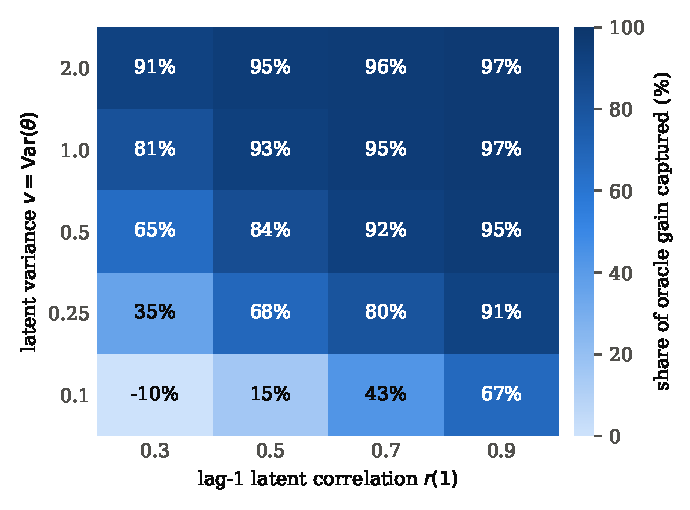
\includegraphics[width=0.62\textwidth]{figures/fig_share_heatmap.pdf}
\caption{Share of the oracle-parameter gain captured by the feasible S1 premium, on the premium-error scale, over the $(v,r(1))$ grid; 500 replications per cell.\label{fig:heatmap}}
\end{figure}

\begin{figure}[H]
\centering
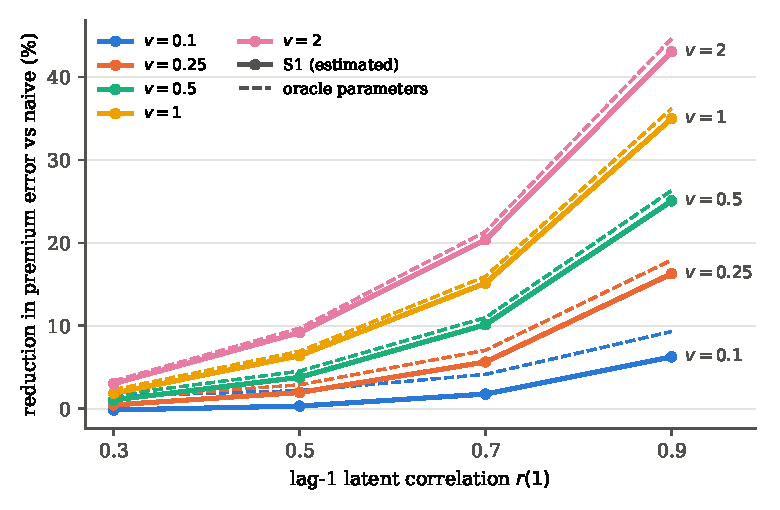
\includegraphics[width=0.7\textwidth]{figures/fig_gain_vs_r1.pdf}
\caption{Relative reduction in premium error versus the naive premium, against the lag-1 latent correlation, for each latent variance $v$. Solid lines with markers: feasible S1 premium; dashed lines: oracle-parameter premium.\label{fig:gain}}
\end{figure}

\begin{figure}[H]
\centering
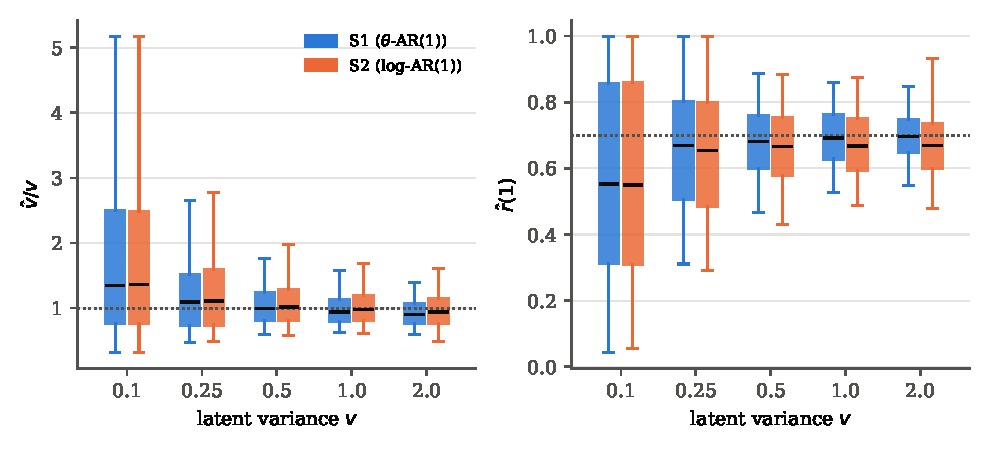
\includegraphics[width=0.9\textwidth]{figures/fig_estimates_box.pdf}
\caption{Sampling distributions of $\hat v/v$ and $\hat r(1)$ for S1 and S2 at $r(1)=0.7$. Boxes show quartiles and whiskers the 5th and 95th percentiles; the dotted line marks the truth.\label{fig:box}}
\end{figure}

\begin{table}[H]
\caption{Estimator variants: share (\%) of the oracle gain captured, and relative reduction (\%) of mean Tweedie deviance versus naive. Hetero.: central cell with $\beta_1=1.5$ and $\beta_0=2$ (more heterogeneous $\mu$).\label{tab:variants}}
\small
\begin{tabular*}{\textwidth}{@{\extracolsep{\fill}}ccccccccccc@{}}
\toprule
 & & \multicolumn{6}{c}{Share of oracle gain (\%)} & \multicolumn{3}{c}{Deviance reduction (\%)} \\
\cmidrule(lr){3-8}\cmidrule(lr){9-11}
$v$ & $r(1)$ & Static & S1 & S1 lag & S1 equal & S2 & NP & Static & S1 & NP \\
\midrule
%BEGIN tab_variants
0.1 & 0.7 & 32 & 43 & 39 & 37 & 43 & $-$44 & 0.04 & 0.04 & $-$0.05 \\
0.25 & 0.7 & 63 & 80 & 78 & 77 & 80 & 56 & 0.31 & 0.36 & 0.24 \\
0.5 & 0.7 & 71 & 92 & 90 & 90 & 92 & 81 & 1.01 & 1.21 & 1.09 \\
1 & 0.7 & 73 & 95 & 92 & 94 & 95 & 88 & 2.80 & 3.24 & 1.96 \\
2 & 0.7 & 72 & 96 & 88 & 95 & 95 & $<-100$ & 6.04 & 6.86 & $-$21.84 \\
0.1 & 0.9 & 76 & 67 & 68 & 59 & 68 & 28 & 0.22 & 0.19 & 0.10 \\
0.25 & 0.9 & 92 & 91 & 90 & 88 & 91 & 78 & 1.07 & 1.05 & 0.91 \\
0.5 & 0.9 & 94 & 95 & 94 & 94 & 95 & 87 & 2.81 & 2.82 & 2.66 \\
1 & 0.9 & 95 & 97 & 94 & 95 & 97 & 80 & 6.81 & 6.79 & $-$17.63 \\
2 & 0.9 & 94 & 97 & 92 & 96 & 98 & 5 & 12.55 & 12.35 & $-$79.89 \\
\multicolumn{2}{c}{hetero.} & 58 & 98 & 102 & 75 & 98 & 95 & 1.18 & 1.47 & $-$1.52 \\
%END tab_variants
\bottomrule
\end{tabular*}
\end{table}

\subsection{Sensitivity Analysis}\label{sec:sensitivity}

Table~\ref{tab:sens} varies one design factor at a time around the central cell, and Table~\ref{tab:null} reports size and power of the tests.

\textbf{Sample size and panel length.} The estimator behaves as Proposition~\ref{prop:asy} predicts. With $I=10{,}000$, S1 captures 98\% of the oracle gain, the $J$ test of S2 has a size of 5.6\%, and the S2 Wald intervals cover $v$ and $r(1)$ in 94\% of replications. With $I=500$, the share falls to 75\%, and the $J$ test over-rejects (12\%). A short panel ($T=3$) reduces the share to 84\% and produces more boundary fits (18\%), whereas $T=10$ raises it to 97\%. With $T=10$, the static Wald test rejects in all but 0.4\% of replications, and the fitted static premium captures only 43\% of the gain, because exchangeability becomes less plausible over a longer window.

\textbf{Dispersion.} Less Tweedie noise ($\phi=5$) raises the share to 98\%, and more noise ($\phi=20$) lowers it to 75\%. The MSE reduction achieved by S1 falls accordingly, from 4.1\% to 0.4\%.

\textbf{Misspecified power parameter.} The moments depend on $p$ only through the nugget scale $q_{it}=\mu_{it}^{p-2}$. With a true $p=1.3$ and a working $p=1.5$, the estimates of $(v,\rho)$ are biased (medians 0.40 and 0.78), and the $J$ test of S2 detects the misspecification in 85\% of replications. Prediction is nevertheless robust: S1 still captures 95\% of the gain. The reverse error is costlier. With a true $p=1.7$ and a working $p=1.5$, part of the Tweedie variance is attributed to $v$ (median $\hat v=2.31$, $\hat\rho=0.16$), the share falls to 58\%, and the $J$ test rejects in only 17\% of replications. Profiling $p$ by the diagonal $J$ statistic (Section~\ref{sec:practical}) locates $p$ correctly on average (median $\hat p=1.35$ and $1.65$), but it is imprecise with $I=2000$ (interquartile range $1.10$--$1.55$ and $1.10$--$1.90$) and recovers only part of the loss. In this design, a working $p$ that is too large is much less harmful than one that is too small.

\textbf{Unbalanced panels and heterogeneity.} With 20\% of policy-years missing at random, the share is 87\%. In the more heterogeneous design ($\beta_1=1.5$), precision weighting matters: the joint GMM captures 98\% of the gain, the equal-weight variant only 75\%.

\textbf{Null designs.} Under a static latent risk, the static Wald test has a size of 6.4\%, and the $J$ test of S3 a size of 6.2\%. The fitted static and S1 premiums capture 99\% and 97\% of the oracle gain, so little is lost by using the evolutionary premium when the truth is static. Under independence, the no-dependence Wald test has a size of 8.8\%, and the static Wald test a size of 7.0\%. Estimating a dependence structure that is absent costs S1 less than 0.01\% of MSE relative to the naive premium (SE 0.003\%). The $J$ tests of S1 and S2 over-reject in this design (11.8\%) because their true parameters lie on the boundary ($\rho=0$), where the $\chi^2$ approximation does not apply \citep{andrews1999}.

\begin{table}[H]
\caption{One-at-a-time sensitivity around the central cell $v=0.5$, $r(1)=0.7$ (500 replications each): median S1 estimates, $J$ rejection rate (\%) of S2, share (\%) of the oracle gain captured, and relative MSE reduction (\%) of S1 versus naive (SE in parentheses).\label{tab:sens}}
\begin{adjustwidth}{-\extralength}{0cm}
\small
\begin{tabular*}{\fulllength}{@{\extracolsep{\fill}}lccccccc@{}}
\toprule
Design & S1 $\hat v$ & S1 $\hat\rho$ & $J$ S2 & Static share & S1 share & S2 share & S1 MSE red. \\
\midrule
%BEGIN tab_sens
Central ($I=2000$, $T=5$, $\phi=10$, $p=1.5$) & 0.50 & 0.68 & 5.8 & 71 & 92 & 92 & 1.50 (0.06) \\
$I=500$ & 0.58 & 0.59 & 12.0 & 63 & 75 & 75 & 1.25 (0.11) \\
$I=10{,}000$ & 0.50 & 0.70 & 5.6 & 72 & 98 & 98 & 1.56 (0.03) \\
$T=3$ & 0.53 & 0.66 & 11.2 & 79 & 84 & 85 & 1.31 (0.06) \\
$T=10$ & 0.48 & 0.70 & 7.8 & 43 & 97 & 97 & 1.59 (0.06) \\
$\phi=5$ & 0.49 & 0.69 & 7.0 & 69 & 98 & 98 & 4.13 (0.09) \\
$\phi=20$ & 0.61 & 0.60 & 6.8 & 63 & 75 & 76 & 0.40 (0.03) \\
True $p=1.3$, working $p=1.5$ & 0.40 & 0.78 & 85.4 & 69 & 95 & 94 & 3.53 (0.08) \\
True $p=1.3$, $p$ profiled (median $\hat p$=1.35) & \multicolumn{3}{c}{---} & 66 & 94 & 94 & 3.51 (0.08) \\
True $p=1.7$, working $p=1.5$ & 2.31 & 0.16 & 17.4 & 62 & 58 & 62 & 0.29 (0.03) \\
True $p=1.7$, $p$ profiled (median $\hat p$=1.65) & \multicolumn{3}{c}{---} & 50 & 63 & 66 & 0.34 (0.03) \\
20\% of years missing & 0.50 & 0.68 & 8.2 & 70 & 87 & 88 & 1.28 (0.05) \\
Heterogeneous $\mu$ ($\beta_1=1.5$) & 0.48 & 0.69 & 6.8 & 58 & 98 & 98 & 3.52 (0.60) \\
%END tab_sens
\bottomrule
\end{tabular*}
\end{adjustwidth}
\end{table}

\begin{table}[H]
\caption{Size and power of the tests (rejection rates in \%, 5\% level, 500 replications, $v=0.5$, $I=2000$, $T=5$), and share (\%) of the oracle gain captured by the fitted static and S1 premiums. Under independence there is no gain to capture.\label{tab:null}}
\begin{adjustwidth}{-\extralength}{0cm}
\small
\begin{tabular*}{\fulllength}{@{\extracolsep{\fill}}lccccccc@{}}
\toprule
Truth & Static Wald & No-dep.\ Wald & $J$ S1 & $J$ S2 & $J$ S3 & Static share & S1 share \\
\midrule
%BEGIN tab_null
Static truth ($\gamma(k)=v$) & 6.4 & 100.0 & 8.0 & 10.8 & 6.2 & 99 & 97 \\
Independence ($\gamma(k)=0$, $k\ge1$) & 7.0 & 8.8 & 11.8 & 11.8 & 19.6 & --- & --- \\
Central design & 50.6 & 99.8 & 5.2 & 5.8 & 48.2 & 71 & 92 \\
%END tab_null
\bottomrule
\end{tabular*}
\end{adjustwidth}
\end{table}

%=================================================================
\section{Discussion and Conclusions}\label{sec:discussion}

This paper develops evolutionary credibility for Tweedie claim costs within a GLM rating structure. Theorem~\ref{thm:main} gives the best linear premium for any second-order stationary latent process. It requires only the autocovariance $\gamma(\cdot)$ and a single nugget constant $a$, and it contains the naive premium and the Tweedie credibility estimator of \citet{ohlsson2006exact} as special cases. For AR(1) dependence, Proposition~\ref{prop:kalman} provides an updating-type recursion with positive weights, a guaranteed positive premium and a bonus cap equal to the persistence parameter. Recency of the weights holds under a mild condition on the evolution of $\mu_t$, but not in general. Because every input of the premium is identified by second moments of standardized residuals, a semi-parametric GMM estimator with closed-form moments, constraints built into the parametrization and stage-1-corrected inference makes the premium operational without distributional assumptions on the latent process.

\textbf{Practical implications.} Four points emerge from the simulation study. First, with estimated parameters the AR(1) premium captures most of the gain that is available to any linear premium, and it never produced a nonpositive premium. Second, a fitted static premium is a safe but conservative choice: it is never materially worse than the naive premium, but it leaves much of the gain unused unless persistence is high. Third, gains should be judged on the premium error, the deviance or rank-based ratemaking metrics rather than on the raw MSE of claim costs, which is dominated by irreducible Tweedie noise. Fourth, the Wald test of a static latent risk has limited power over a five-year window when persistence is very high, but in exactly those cases static and evolutionary premiums nearly coincide, so the cost of a wrong decision is small.

\textbf{Limitations.} The premium is linear and therefore not the exact Bayesian predictor. Its optimality is restricted to linear rules, and higher-order features of the latent law (e.g., tail dependence) do not enter it. Second-moment inference is sensitive to the heavy tails of squared Tweedie residuals: when the latent variance is large, Wald intervals for $v$ under-cover and the $J$ test over-rejects. The policyholder-level bootstrap repairs the under-coverage caused by a weak signal, but not the under-coverage caused by heavy tails. Robust (e.g., trimmed or median-based) moment conditions are a natural remedy. Prediction is much less affected than inference. With $T=5$, the $J$ test cannot discriminate between $\theta$-scale and log-scale AR(1) dependence, although this distinction turned out to be immaterial for prediction. The power parameter $p$ must be chosen or profiled, and we have not yet applied the method to real data.

\textbf{Extensions.} Natural next steps are as follows:
\begin{itemize}
\item an application to a longitudinal policy-level portfolio with five or more years, such as the Wisconsin Local Government Property Insurance Fund data used by \citet{frees2016multivariate};
\item robustness studies with latent processes that share $\gamma(\cdot)$ but differ in higher-order dependence, for example gamma autoregressions or copula-based Markov chains with tail dependence;
\item an exact-Bayes benchmark by particle filtering, to quantify the cost of linearity;
\item comparisons with machine-learning predictors that use lagged claims, such as gradient boosting with Tweedie loss, evaluated with ordered Lorenz curves and Gini indices;
\item hierarchical \citep{taylor2018}, higher-order and long-memory \citep{pinquet2020} latent structures, all of which fit Theorem~\ref{thm:main} and the GMM framework of Section~\ref{sec:estimation} without modification.
\end{itemize}

%=================================================================
\vspace{6pt}

\authorcontributions{[To be completed by the authors.]}

\funding{[To be completed by the authors.]}

\institutionalreview{Not applicable.}

\informedconsent{Not applicable.}

\dataavailability{No new data were created. The simulation code (Python) that reproduces all tables and figures is available in the authors' repository [link to be added].}

\acknowledgments{This article is based on the first author's MSc project at Simon Fraser University \citep{kang2026}, supervised by the second author. [GenAI statement to be confirmed by the authors: During the preparation of this manuscript, the authors used Claude (Anthropic) to assist with drafting text, implementing the simulation code and preparing tables and figures. The authors have reviewed and edited the output and take full responsibility for the content of this publication.]}

\conflictsofinterest{The authors declare no conflicts of interest.}

\abbreviations{Abbreviations}{%
The following abbreviations are used in this manuscript:\\

\noindent
\begin{tabular}{@{}ll}
AR(1) & first-order autoregressive \\
BLP & best linear predictor \\
GLM & generalized linear model \\
GMM & generalized method of moments \\
MD & minimum distance \\
MSE & mean squared error \\
NP & nonparametric (autocovariance) \\
\end{tabular}
}

%=================================================================
\appendixtitles{yes}
\appendixstart
\appendix
\section{Proofs}\label{app:proofs}

\textbf{Proof of Proposition~\ref{prop:kalman}.}
\emph{(a)} Let $\hat x_t$ be the best linear predictor of $x_t$ given $(1,e_1,\dots,e_{t-1})$, and let $V_t$ be its MSE. Then $\hat x_1=\E x_1=0$ and $V_1=v$. The innovation $e_t-\hat x_t=(x_t-\hat x_t)+\varepsilon_t$ has variance $V_t+d_t$, because $\varepsilon_t$ is uncorrelated with $x_t$ and with the past. Projecting $x_t$ on the innovation gives $\hat x_{t\mid t}=\hat x_t+K_t(e_t-\hat x_t)$, with MSE $(1-K_t)V_t$. Since $\eta_t=x_{t+1}-\rho x_t$ is uncorrelated with $(e_1,\dots,e_t)$, we get $\hat x_{t+1}=\rho\hat x_{t\mid t}$ and $V_{t+1}=\rho^2(1-K_t)V_t+\Var\eta_t$. Finally, $\varepsilon_{T+1}$ is uncorrelated with $(e_1,\dots,e_T)$, so the best linear predictor of $e_{T+1}$ is $\hat x_{T+1}$. The best linear predictor is unique, so it coincides with \eqref{eq:premium}. See \citet[Proposition~12.2.2]{brockwell1991} for the general wide-sense Kalman recursions.

\emph{(b)} Unrolling $\hat x_{t+1}=\rho(1-K_t)\hat x_t+\rho K_te_t$ from $\hat x_1=0$ gives the stated coefficients. Since $V_1=v>0$, $V_{t+1}\ge(1-\rho^2)v>0$ and $0<d_t<\infty$, we have $K_t\in(0,1)$, so $w_t>0$ when $\rho>0$.

\emph{(c)} Summing the coefficients of $\hat x_{t+1}$ gives $S_t=\rho(1-K_t)S_{t-1}+\rho K_t$. If $0\le S_{t-1}<1$, then $(1-K_t)S_{t-1}+K_t=1-(1-K_t)(1-S_{t-1})\in(0,1)$, hence $0<S_t<\rho$. Induction from $S_0=0$ completes the proof.

\emph{(d)} Since $Z_t\ge0$, we have $e_t\ge-1$. By (b), $\sum_tw_te_t\ge-S_T$, with equality if and only if $Z_1=\dots=Z_T=0$. The bound follows from (c).

\emph{(e)} Let $\lambda=1/v$, $u_t=V_t/v$ and $\delta_t=\lambda d_t$. Then $u_1=1$, $K_t=u_t/(u_t+\delta_t)$ and $u_{t+1}=\rho^2h(u_t,\delta_t)+1-\rho^2$ with $h(x,y)=xy/(x+y)$. We show by induction that $u_t/\lambda$ is nonincreasing in $\lambda$. This is clear for $t=1$. Since $h$ is homogeneous of degree one, $u_{t+1}/\lambda=\rho^2h(u_t/\lambda,d_t)+(1-\rho^2)/\lambda$. The function $h$ is nondecreasing in its first argument, so the claim follows. Hence $K_t=\{1+d_t/(u_t/\lambda)\}^{-1}$ is nonincreasing in $\lambda$, i.e., nondecreasing in $v$, and so is $w_T=\rho K_T$. Finally, $S_t=\rho\{S_{t-1}+K_t(1-S_{t-1})\}$ is nondecreasing in both $S_{t-1}$ and $K_t$ because $S_{t-1}<1$, so $S_T$ is nondecreasing in $v$. Replacing every $\mu_t$ by $c\mu_t$ multiplies every $d_t$ by $c^{p-2}$, which is equivalent to replacing $v$ by $c^{2-p}v$.

\emph{(f)} From (b), $w_{t-1}/w_t=\rho K_{t-1}(1-K_t)/K_t=\rho K_{t-1}\delta_t/u_t$. Moreover, $(1-K_{t-1})u_{t-1}=K_{t-1}\delta_{t-1}$, so $u_t=\rho^2K_{t-1}\delta_{t-1}+1-\rho^2$. Hence $w_{t-1}<w_t$ if and only if
\[
\rho K_{t-1}\{(1-\rho)\delta_{t-1}+(\delta_t-\delta_{t-1})\}<1-\rho^2 .
\]
By induction, $u_t\le1$ for all $t$, since $u_{t+1}=\rho^2h(u_t,\delta_t)+1-\rho^2$ and $h(u_t,\delta_t)<u_t$. Therefore $K_{t-1}\delta_{t-1}=h(u_{t-1},\delta_{t-1})<1$ and $K_{t-1}<1$, and the left-hand side is smaller than $\rho(1-\rho)+\rho(\delta_t-\delta_{t-1})^+$. This is at most $1-\rho^2$ whenever $(\delta_t-\delta_{t-1})^+\le(1-\rho)/\rho$, that is, $d_t-d_{t-1}\le v(1-\rho)/\rho$. The counterexample in the main text violates this condition.

\emph{(g)} As $\rho\to0$, $\bc_T\to\boldsymbol0$ while $\Gamma_T+D_T\to vI+D_T$ stays nonsingular. As $\rho\to1$, $\Gamma_T\to v\bone\bone^\top$ and $\bc_T\to v\bone$, and $(\Gamma_T+D_T)^{-1}$ is continuous because the limit is positive definite. With $d_t\equiv d$, the map $f(u)=\rho^2h(u,\delta)+1-\rho^2$ satisfies $0<f'(u)=\rho^2\delta^2/(u+\delta)^2<\rho^2$, so $u_t$ converges to the unique fixed point $u^\ast$. The fixed point solves $u^2+(1-\rho^2)(\delta-1)u-(1-\rho^2)\delta=0$, and $u^\ast$ is its positive root. The limiting weights follow from (b) with $K_s\to K^\ast$, and the sum converges by dominated convergence, since $w_{T+1-j}\le\rho^j$.

\section{Exact Mean Squared Error of Linear Premiums}\label{app:mse}

Let $P=\mu_{T+1}(1+\bw^\top\be_T)$, where $\bw$ is any weight vector that depends on covariates only. Then $Z_{T+1}-P=\mu_{T+1}(e_{T+1}-\bw^\top\be_T)$, and Lemma~\ref{lem:moments} gives
\begin{equation}\label{eq:exactmse}
\E[(Z_{T+1}-P)^2\mid\bx]=\mu_{T+1}^2\big\{v+a\mu_{T+1}^{p-2}-2\bw^\top\bc_T+\bw^\top(\Gamma_T+D_T)\bw\big\}.
\end{equation}
Averaging \eqref{eq:exactmse} over the covariate distribution (here over $2\times10^6$ simulated policies) gives the exact population MSE of the naive premium ($\bw=\boldsymbol0$), of the oracle-parameter premium ($\bw=(\Gamma_T+D_T)^{-1}\bc_T$) and of every exchangeable premium. The \emph{best exchangeable} premium minimizes the population MSE over the static credibility constant, using the true $a$ and $\bmu$. Moreover, if $P$ is any function of the training data, then $\E[Z_{T+1}-\mu_{T+1}\theta_{T+1}\mid\boldsymbol\theta,\mathcal{F}_T]=0$ implies
\[
\E(Z_{T+1}-P)^2=\E(\mu_{T+1}\theta_{T+1}-P)^2+\E\big[a\mu_{T+1}^{p}\big].
\]
Differences in out-of-sample MSE between premiums therefore equal differences in the \emph{premium error} $\E(\mu_{T+1}\theta_{T+1}-P)^2$. The premium error excludes the irreducible Tweedie noise and has a much smaller Monte Carlo variance.

\section{Computational Details}\label{app:computation}

Tweedie variates are generated from the compound Poisson--gamma representation: $N\sim\mathrm{Poisson}(\mu^{2-p}/\{\phi(2-p)\})$, and given $N$, $Z\sim\mathrm{Gamma}(N(2-p)/(p-1),\ \phi(p-1)\mu^{p-1})$, with $Z=0$ if $N=0$. Stage 1 uses Fisher scoring for the Tweedie quasi-score. Stage 2 starts from equal weights and recomputes the precision weights three times from $(\hat\gamma(0),\hat a)$, floored at $0.02$. $G_\beta$ is obtained by central differences with step $10^{-5}$ and the weights held fixed. The minimum-distance problems \eqref{eq:md} are solved by BFGS from three starting values derived from the NP estimates. The Proposition~\ref{prop:kalman} recursion agrees with the direct solve of \eqref{eq:premium} to $10^{-11}$, and the simulated MSE of the oracle-parameter premium agrees with \eqref{eq:exactmse} within Monte Carlo error. The code is organized as \texttt{tweedie\_gmm.py} (estimator, tests and premiums), \texttt{sim.py} (simulation design), \texttt{test\_core.py} (unit tests) and \texttt{make\_tables.py} (tables and figures).

%=================================================================
\begin{adjustwidth}{-\extralength}{0cm}
\reftitle{References}
\bibliography{refs}
\PublishersNote{}
\end{adjustwidth}
\end{document}
